\section{Kvalitativ analyse}
\label{section:kvalitativ_analyse} 

\subsection{Stegvis-deduktiv induktiv metode}
Analysen av datamaterialet er blitt utført etter en \textit{stegvis-deduktiv induktiv} metodisk tilnærming, som beskrevet av \citet{Tjora}, se figur \ref{SDI}. De oppadgående pilene beskriver det induktive arbeidet, i den forstand at man jobber fra data mot teori, mens de nedadgående pilene beskriver den deduktive prosessen, hvor man sjekker fra det mer teoretiske mot det mer empiriske. 

\begin{figure}[H]
\centering
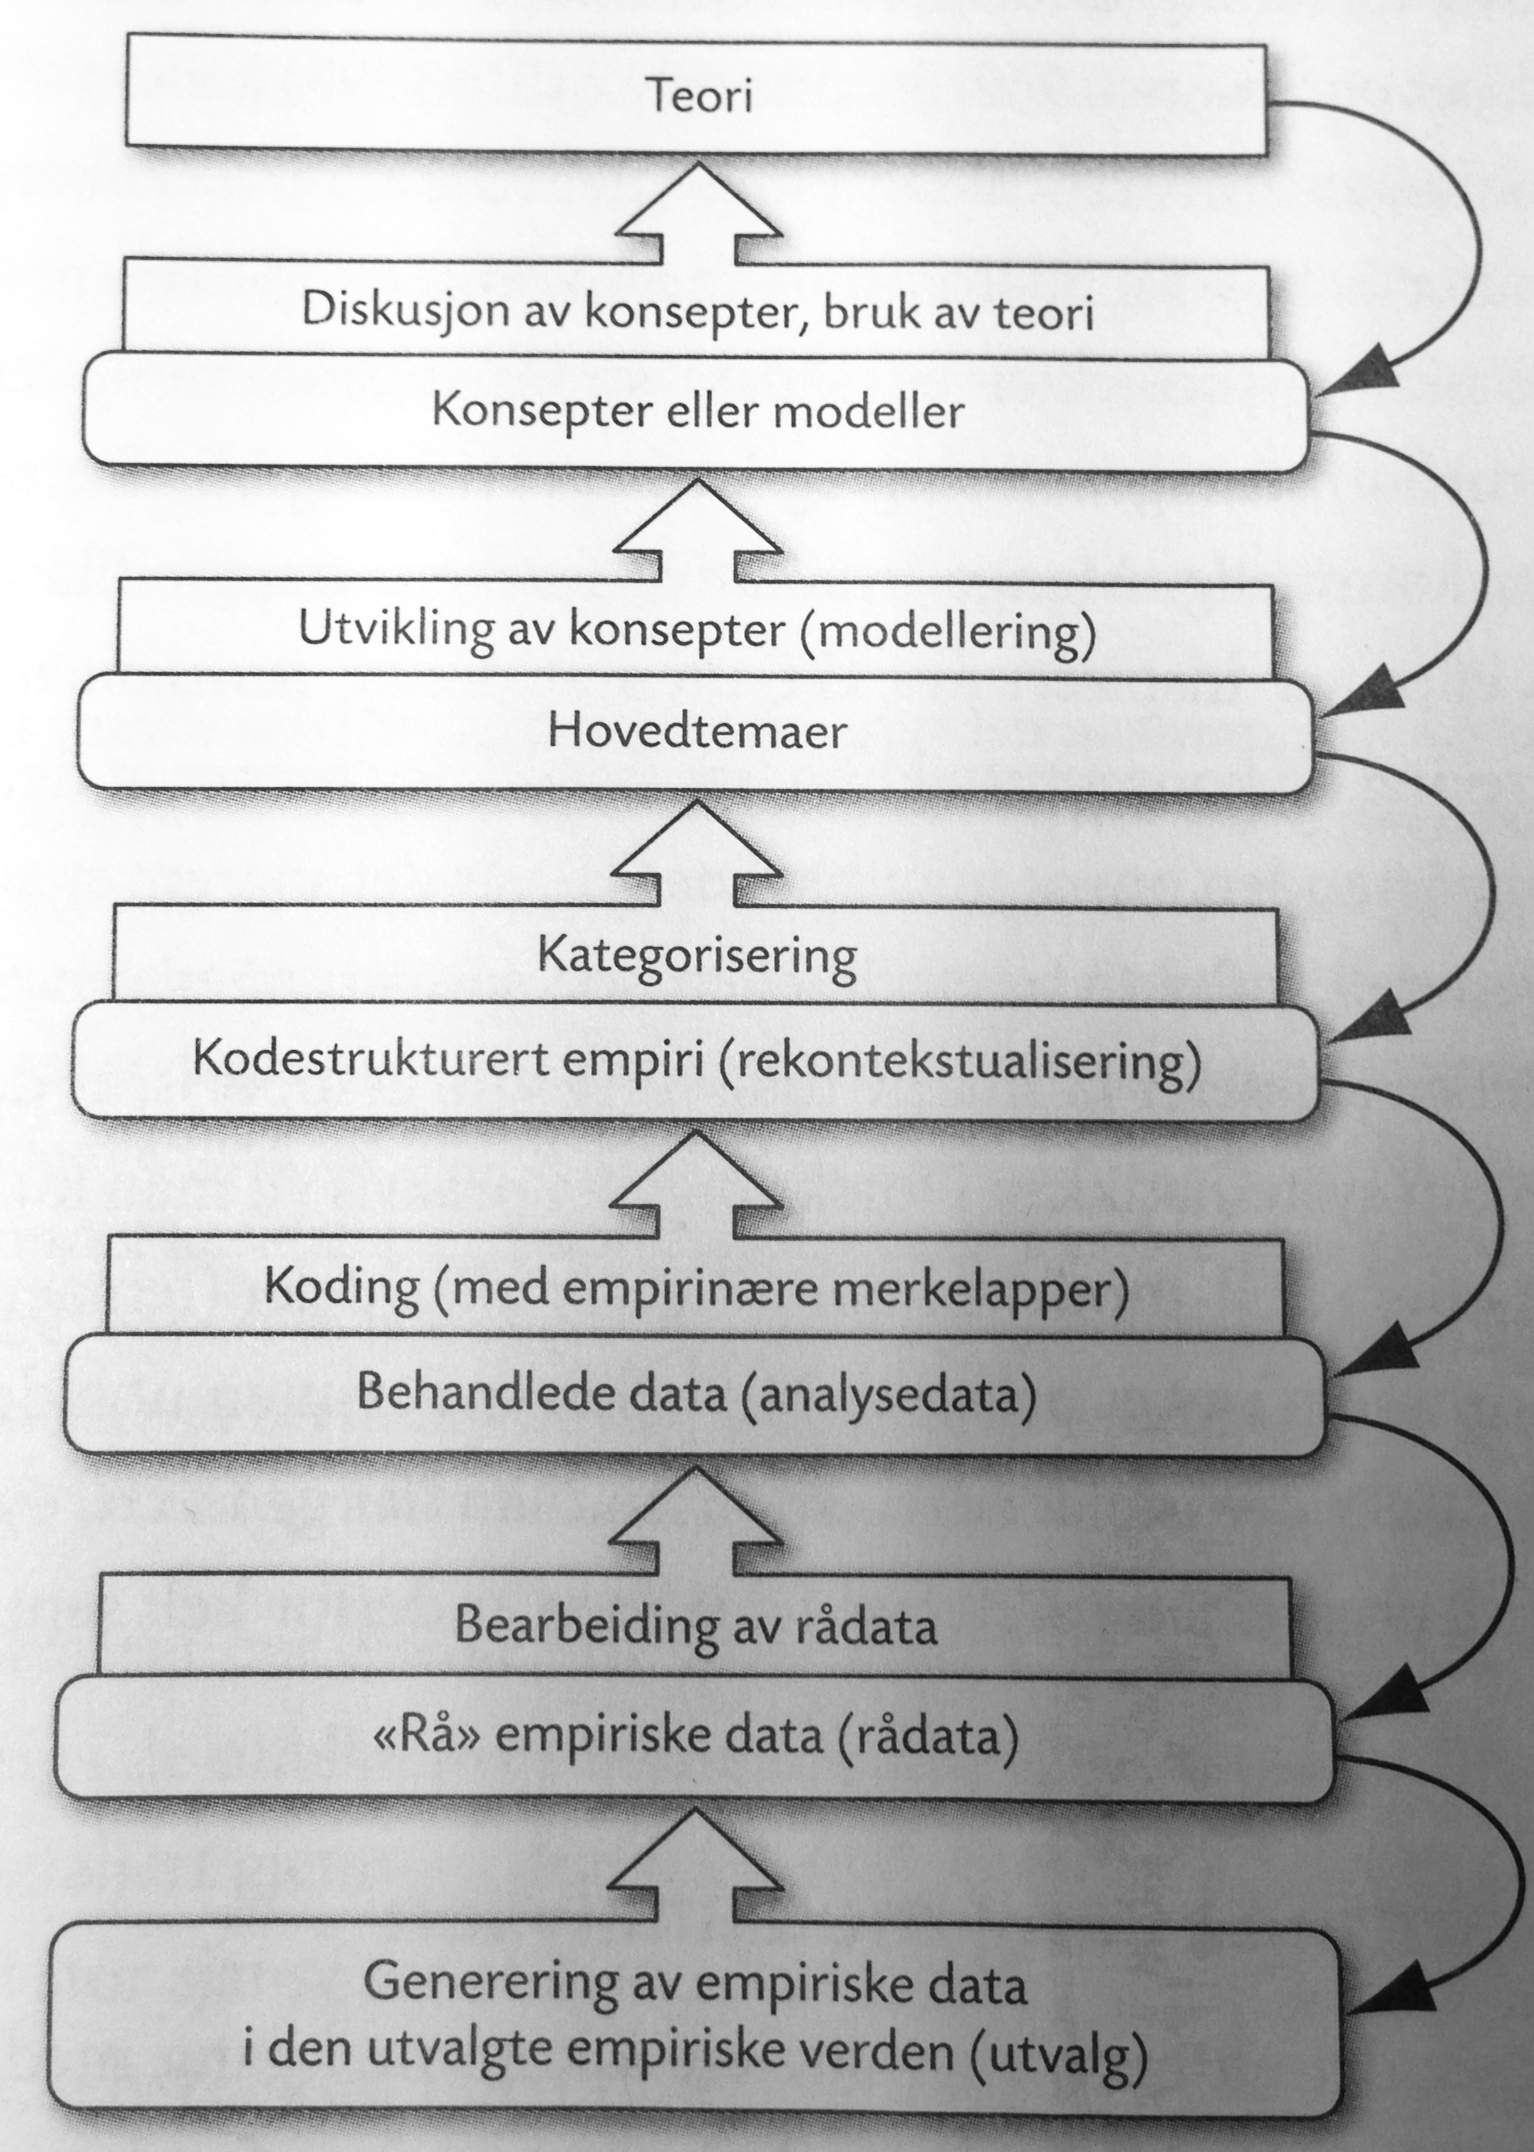
\includegraphics[scale=0.1]{SDI.jpg}
\caption{Stegvis-deduktiv induktiv metode \citep{Tjora})}
\label{SDI}
\end{figure}

\noindent
Feltnotatene fra første observasjonsperiode ble transkribert, og deretter kodet og kategorisert ved bruk av dataprogrammet RStudio \citep{Rstudio}. Kodingen av observasjonsdataene resulterte i nærmere 100 koder, og forskerne jobbet på denne måten induktivt med materialet. Det høye antallet koder forklares ved at forskerne genererte detaljerte, \textit{tekstnære}, koder fra en stor mengde data \citep{Tjora}. For å kunne luke ut empiri som ikke var relevant for videre forskning ble kodene kategorisert i 11 kategorier. Dette ga forskerne en større, og mer strukturert oversikt over forskningsområdet, og de formulerte forskningsspørsmål som det videre arbeidet søkte svar på. Forskningsarbeidet beveget seg dermed fra konsept-utviklingsfasen til en ny runde med generering av empiriske data. Feltnotatene fra andre observasjonsperiode ble kodet og kategorisert, med nærmere 50 koder, og 5 kategorier. Etter observasjonsperioden utpekte det seg dermed sentrale temaer som videre formet intervjuguidene. Lydopptakene fra intervjuene ble transkribert og brukt som støtte til observasjonsdataene, for å utdype, sammenligne og avdekke sprik mellom forskernes og informantenes oppfatninger. Avslutningsvis forsøkte forskerne å konseptualisere og diskutere avdekkede funn i lys av relevant teori. 


\subsection{Datamaterialets kvalitet}
Ulike forhold kan påvirke datamaterialets kvalitet, og ofte benyttes de tre kriteriene \textit{reliabilitet}, \textit{validitet} og \textit{generaliserbarhet} som indikatorer på kvalitet \citep{Tjora}. Reliabilitet omhandler hvorvidt forskerne selv kan ha preget forskningsarbeidet, og både \citet{Oates} og \citet{Tjora} understreker at fullstendig nøytralitet er umulig. 

Det kan være vanskelig å generalisere kvalitativ forskning, da antallet informanter blir ubetydelig lite i forhold til hele populasjonen. 



- triangulering

- validitet

